\documentclass[10pt,twocolumn,letterpaper]{article}

\usepackage{packages/cvpr}
\usepackage{times}
\usepackage{epsfig}
\usepackage{graphicx}
\usepackage{amsmath}
\usepackage{amssymb}
\usepackage{caption}
\usepackage{tikz}    
\usepackage{makecell} 
\usepackage{float}    

% Include other packages here, before hyperref.

% If you comment hyperref and then uncomment it, you should delete
% egpaper.aux before re-running latex.  (Or just hit 'q' on the first latex
% run, let it finish, and you should be clear).
\usepackage[pagebackref=true,breaklinks=true,letterpaper=true,colorlinks,bookmarks=false]{hyperref}

% Tikz imports and setup for flowcharts
\usetikzlibrary{shapes.geometric, arrows}
\tikzstyle{block} = [rectangle, rounded corners, minimum width=1.7cm, minimum height=0.5cm,text centered, draw=black]
\tikzstyle{arrow} = [thick,->,>=stealth]

\cvprfinalcopy % *** Uncomment this line for the final submission

\def\cvprPaperID{****} % *** Enter the CVPR Paper ID here
\def\httilde{\mbox{\tt\raisebox{-.5ex}{\symbol{126}}}}

% Pages are numbered in submission mode, and unnumbered in camera-ready
\ifcvprfinal\pagestyle{empty}\fi
\begin{document}

%%%%%%%%% TITLE
\title{CLIP Hackathon Task \\ \normalsize\bfseries Advanced Topics in Deep Learning: The Rise of Transformers}

\author{Raul Singh\\
Politecnico di Milano\\
{\tt\small raul9.singh@mail.polimi.it}
\and
Davide Rigamonti\\
Politecnico di Milano\\
{\tt\small davide2.rigamonti@mail.polimi.it}
}

\maketitle
%\thispagestyle{empty}

%%%%%%%%% ABSTRACT
\begin{abstract}
   TODO The ABSTRACT should be self-contained and explain what the paper is about. Usually abstracts are no longer than 300 words. You should state what are the main contributions of your work and tempt the reader to continue to read your paper. A good abstract briefly describes your problem, approach, and key results. This document is based on the CVPR submission template, and it has been adapted to submit a technical report of a project of the Deep Learning and Image Classification course.
\end{abstract}

%%%%%%%%% BODY TEXT
%------------------------------------------------------------------------
\section{Introduction}
This is a project that has been developed in the context of the \textit{Advanced Topics in Deep Learning: The Rise of Transformers} course held at \textit{Politecnico di Milano} and supervised by Professor Matteo Matteucci.
The initial assignment was carried out as a one-day hackathon held at Politecnico on the 1st of February 2023.
Then, groups composed of M.Sc.\ students were asked to improve upon their initial design in order to overtake their baseline performance by means of creative additions and overall improvements.

Groups were expected to implement their designs from scratch, without copy-pasting pieces of code from the assigned references.
The language recommended for the implementation is \href{https://www.python.org/}{Python}, with the addition of the \href{https://www.tensorflow.org/}{TensorFlow}/\href{https://keras.io/}{Keras} libraries.

We used \href{https://jupyter.org/}{Jupyter Notebooks} as a way to organize our work into self-contained and meaningful subtasks, we utilized \href{https://www.kaggle.com/}{Kaggle} and \href{https://colab.research.google.com}{Google Colab} as means to access computing power to train our models when local resources weren't available to us and lastly, we chose \LaTeX~to write the final report.

\subsection{Task}
The central challenge for this project is to develop a functional implementation of the \href{https://openai.com/}{OpenAI} \textbf{CLIP} model for the main task of \textbf{image retrieval} in a biomedical application.
The following \href{https://openai.com/research/clip}{blog post} and \href{https://arxiv.org/pdf/2103.00020.pdf}{research paper} were given in the assignment as a starting point for understanding the principles of the model, in addition to the information already given by Professor Giacomo Boracchi during the course's frontal lectures.

\subsubsection*{CLIP Principles}
In short, \textbf{CLIP} stands for \textbf{C}ontrastive \textbf{L}anguage-\textbf{I}mage \textbf{P}re-training, and it is composed by two \textit{encoders} (one dedicated to images and one for text) which are trained to minimize the loss computed as the \textit{cosine similarity} of the embedded image pairs.

This peculiar pre-training technique enables the model to achieve relevant performance metrics on a wide array of zero-shot tasks (such as classification) while using a fraction of the dataset of other popular deep learning models performing the same task.

\subsection{Dataset Analysis}

The dataset provided is a \textit{simplified} version of the \href{https://link.springer.com/chapter/10.1007/978-3-030-01364-6_20}{\textbf{ROCO} dataset} (\textbf{R}adiology \textbf{O}bjects in \textbf{CO}ntext) which consists of \textit{83275} elements composed of:

\begin{itemize}
   \item A low resolution image that has been reduced in size.
   \item A corresponding textual caption that describes the image.
   \item A set of concept labels that characterizes the attributes of the image.
\end{itemize}

There are \textit{80813} unique captions as most of them are present in the database only one time, the most common caption appears in \textit{261} images.

Images can have from \textit{1} to \textit{50} concepts associated to them from a total of \textit{8374} concepts, averaging around \textit{5} concepts per image.

Concepts can have from \textit{2} to \textit{25989} images associated to them from a total of \textit{83275} concepts, averaging around \textit{47} images per concept.

\begin{figure}[H]
   \centering
   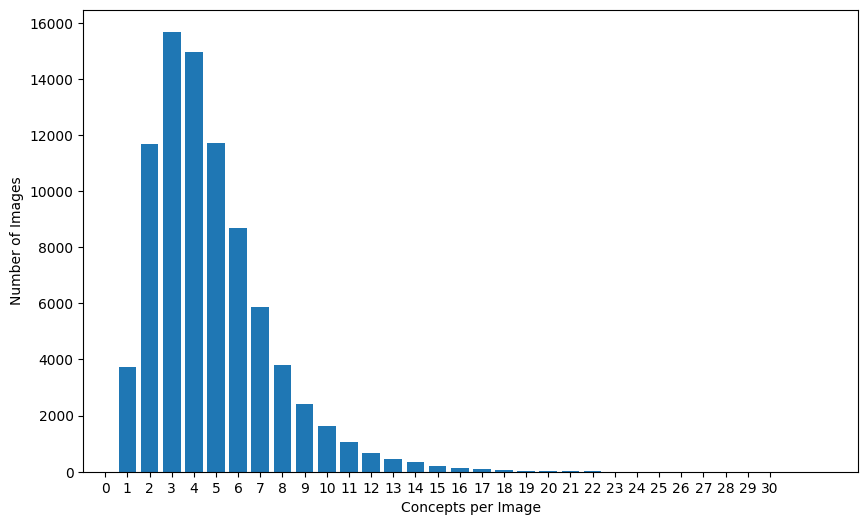
\includegraphics[width=1\linewidth]{img/Data_Exploration_2.png}
   \caption{\textit{Concepts per Image}}
\end{figure}
\begin{figure}[H]
   \centering
   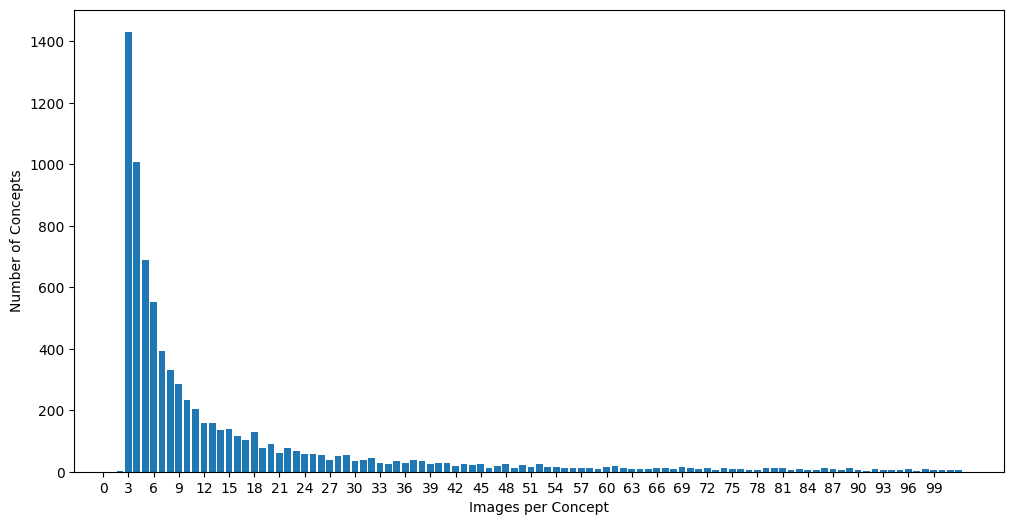
\includegraphics[width=1\linewidth]{img/Data_Exploration_3.png}
   \caption{\textit{Images per Concept}}
\end{figure}


%------------------------------------------------------------------------
\section{Hackathon Results}
The self-imposed goal for the hackathon was to build a CLIP model capable of performing image retrieval, thus we initially left out the portion of data regarding concepts and labels.

Unfortunately we didn't manage to create a functioning notebook in the allotted time.
However, we can still consider ourselves satisfied with our work, since right after the event we noticed that we were just a small change away to obtain a fully working CLIP model.

\subsection{Initial Intuition}
During the hackathon, we opted for splitting our efforts into two separate tasks: model creation and data gathering.
We created 2 preliminary notebooks that tackled the defined tasks, these notebooks were then joined together into a single notebook, considered the final product for the hackathon.

\subsubsection{Data Gathering}
Since the given dataset was problematic to handle due to its dimension and its uncommon compression encoding, part of our efforts were dedicated to create a proper \textit{data pipeline} to feed the model.

The preliminary data gathering pipeline loads captions and images separately, performing different preprocessing for both of them (using the \textit{transformer custom standardization function} seen during lectures for textual data, while performing \textit{resizing} and \textit{normalization} for image pixel data).
The captions are then vectorized using a \href{https://www.tensorflow.org/api_docs/python/tf/keras/layers/TextVectorization}{Keras text vectorization layer}, all the elements are split manually into train, test and validation sets and stored into Python lists.

Various visualizations of the imported images and data were added to ensure the correctness of the loading process.

\subsubsection{Model Creation}
For the preliminary model we decided to implement the encoders from scratch in order to avoid adding useless complexity to our prototype.

For the image encoding we defined a simple CNN composed by 3 \href{https://www.tensorflow.org/api_docs/python/tf/keras/layers/Conv2D}{convolutional layers} with increasing neuron count (from 64 to 256 neurons) with the inclusion of \href{https://www.tensorflow.org/api_docs/python/tf/keras/layers/BatchNormalization}{batch normalization layers}.
At the top of the convolutional section we added a \href{https://www.tensorflow.org/api_docs/python/tf/keras/layers/Flatten}{flattening layer} followed by two \href{https://www.tensorflow.org/api_docs/python/tf/keras/layers/Dense}{dense layers} to obtain a final embedding of size 128.
All of the hidden layers have \href{https://www.tensorflow.org/api_docs/python/tf/keras/layers/ReLU}{ReLU} activation functions.

For the text encoding we used a \textit{transformer encoder block} that was presented during the course lectures, which makes use of \href{https://www.tensorflow.org/api_docs/python/tf/keras/layers/MultiHeadAttention}{multi-head attention}, \href{https://www.tensorflow.org/api_docs/python/tf/keras/layers/LayerNormalization}{layer normalization} and \href{https://www.tensorflow.org/api_docs/python/tf/keras/layers/Dropout}{dropout} layers; at the end of the block there are 2 \textit{dense layers} to obtain a final embedding of size 128.
Before being fed to the encoder block, inputs pass through a double \href{https://www.tensorflow.org/api_docs/python/tf/keras/layers/Embedding}{embedding layer} that implements \textit{positional embedding} by addition.

The complete model routes the two inputs (image and text) to their respective encoders, normalizes the resulting embeddings and obtains the \textit{logits} by applying the formula outlined in the OpenAI paper: $logits = (I_e \cdot T_e^{\top})e^t$.
Then, the individual losses are calculated by means of \href{https://www.tensorflow.org/api_docs/python/tf/keras/losses/CategoricalCrossentropy}{categorical cross-entropy} and are averaged to obtain the final loss.

\subsection{Idea Refining}
As mentioned before, the very last notebook obtained at the end of the hackathon didn't work correctly as there were some small discrepancies between the sizes of the expected inputs vs.\ the actual inputs, and we were trying to apply \textit{categorical cross-entropy} utilizing numeric variables that were not \textit{one-hot encoded}.

The day after the hackathon took place we dedicated some of our time to slightly refine the final product obtained in order to have a functioning model.
By adapting the structure of our network to the input data, fixing minor conflicts related to typing and employing \href{https://www.tensorflow.org/api_docs/python/tf/keras/losses/SparseCategoricalCrossentropy}{sparse categorical cross-entropy} instead of \textit{categorical cross-entropy}, we managed to obtain a working CLIP implementation.

Due to the inefficient loading technique we weren't able to hold the entirety of the dataset and the model in memory, thus we couldn't test it properly.
However, by considering a fraction of the dataset and training the model on it for around 10 epochs, we noticed that the results were quite scarce as the loss would not get any lower after the first few epochs.
When considering a top-k image-retrieval task on the training dataset with an exact caption as a query, the target image was only occasionally present in the top-10 matched results, and never in the top-5.

The reported results of this step are based on empirical observation as we did not have a proper evaluation system for this task yet.
This is due to the fact that our main goal for the hackathon was to produce a functioning model, not evaluate its performance.


%------------------------------------------------------------------------
\section{Post-Hackathon Improvements}
This section is dedicated to exploring all the improvements (successful and non) that were performed in the months following the initial hackathon challenge.
Some of these improvements are strictly related to the model structure and performance, while others are centered around \textit{data exploration}, \textit{data gathering} and \textit{model evaluation}.

\subsection{Loss Function}
We decided to reimplement the loss function and how it is integrated inside the CLIP model from scratch as we previously made use of \href{https://www.tensorflow.org/api_docs/python/tf/keras/layers/Lambda}{TensorFlow lambda layers} to perform mathematical operations.
We noticed that these layers were causing problems in both the gradient calculation process and during import/export operations.

The approach we took for the new loss was quite radical as we decided to delve into the \href{https://www.tensorflow.org/api_docs/python/tf/keras/Model}{Keras model} by \textit{overriding} the \texttt{train\char`_step} and \texttt{text\char`_step} in order to have more control on how the model calculates loss and how it performs its backpropagation process.
Although we modified the overall structure of the model, the mathematical essence of the loss function remains the same as the one defined in the reference OpenAI paper.

\subsection{Lazy Loading}
It was previously mentioned that the size of the complete dataset was a critical factor that needed to be taken into account at some point.

By implementing a \textit{lazy loading} interface utilizing the \href{https://www.tensorflow.org/api_docs/python/tf/data/Dataset}{TensorFlow dataset class} and exploiting the \textit{map/reduce paradigm} with \textit{lambda functions} we were able to load the actual pixel data of images from their image path only when needed.
We wrapped this operation inside a custom function called \texttt{create\char`_dataset} that exposes a general interface which allows for parametrization of the dataset creation procedure through parameters that influence \textit{batching}, \textit{shuffling}, \textit{dataset structure}, \textit{caching} and other aspects.

At this point we noticed that the vectorization for the captions was causing a minor \textit{data leakage} from the test set to the train set, we corrected the mistake and implemented a new splitting function by wrapping the \href{https://scikit-learn.org/stable/modules/generated/sklearn.model_selection.train_test_split.html}{scikit-learn train\_test\_split function} inside a custom function to also manage validation splits.

\subsection{Pre-Trained Models}
As previously explained, our implementation of the model was completely from scratch. At this point we encountered a performance bottleneck, impeding any further enhancement of the model. This was probably due to the huge amount of parameters in the model, which were quite a challenging task to train from scratch, even considering our large dataset.

As shown during the course lectures, we decided to try to leverage a \textit{pre-trained} model for both our image and text encoder and perform \textit{transfer learning}.

\subsubsection{Image Encoder}
For the image encoder, we chose to utilize a \href{https://github.com/facebookresearch/ConvNeXt}{ConvNeXt} network via the \href{https://keras.io/api/applications/}{Keras Applications API}, specifically the \href{https://keras.io/api/applications/convnext/#convnexttiny-function}{ConvNeXtTiny} variant, known for its compact size yet commendable performance.
We made this selection based on two primary reasons: firstly, to opt for a reasonably sized and efficient CNN to mitigate the risk of overfitting, and secondly, due to our past projects demonstrating impressive results with this network, making it a logical starting point.

Further in the project development, we tried most of the CNNs available on the \href{https://keras.io/api/applications/}{Keras Applications API}, and achieved a substantial improvement using the \href{https://keras.io/api/applications/efficientnet_v2/#efficientnetv2s-function}{EfficentNetV2S} over the \textit{ConvNeXtTiny}.

\subsubsection{Text Encoder}
As for the text encoder, we employed \href{https://huggingface.co/docs/transformers/model_doc/bert}{BERT} as our preferred \textit{text transformer}.
We initially utilized the base version of the transformer as a foundation.

Importing and integrating the model as a layer within our architecture posed a challenge, given that most methods are designed for standalone use of these models.
In the end we successfully overcame this obstacle thanks to the \href{https://www.tensorflow.org/hub}{\texttt{tensorflow\_hub}} module, importing BERT as a \href{https://www.tensorflow.org/hub/api_docs/python/hub/KerasLayer}{\texttt{KerasLayer}} and seamlessly incorporating it into our model.

\subsection{Embedding Projection}
As previously explained, our architecture comprises the following components:
\begin{itemize}
   \item an \textit{image encoder} followed by a 2-layer dense neural network
   \item a \textit{text encoder} followed by a 2-layer dense neural network
\end{itemize}
The purpose of the 2-layer dense network is to project the \textit{high-level features} extracted from the encoders into a shared embedding space.
In an effort to enhance this projection, we engaged in thorough experimentation.
After extensive tinkering, we settled on a 2-layer dense network with \textit{dropout} incorporated in the middle, along with a \textit{residual connection} linking the two dense layers, culminating in \href{https://keras.io/api/layers/normalization_layers/layer_normalization/}{layer normalization}.

We also explored various activation functions, starting with \href{https://keras.io/api/layers/activation_layers/relu/}{ReLU} and subsequently testing \href{https://www.tensorflow.org/api_docs/python/tf/keras/activations/gelu}{GELU}, \href{https://www.tensorflow.org/api_docs/python/tf/nn/silu}{SiLU}, and \href{https://www.tensorflow.org/api_docs/python/tf/nn/selu}{SELU}. Ultimately, SELU demonstrated a significant improvement, prompting us to adopt it for the projection.

Both dense layers were configured with 128 neurons, resulting in a 128-dimensional embedding space.

\begin{figure}[H]
   \centering
   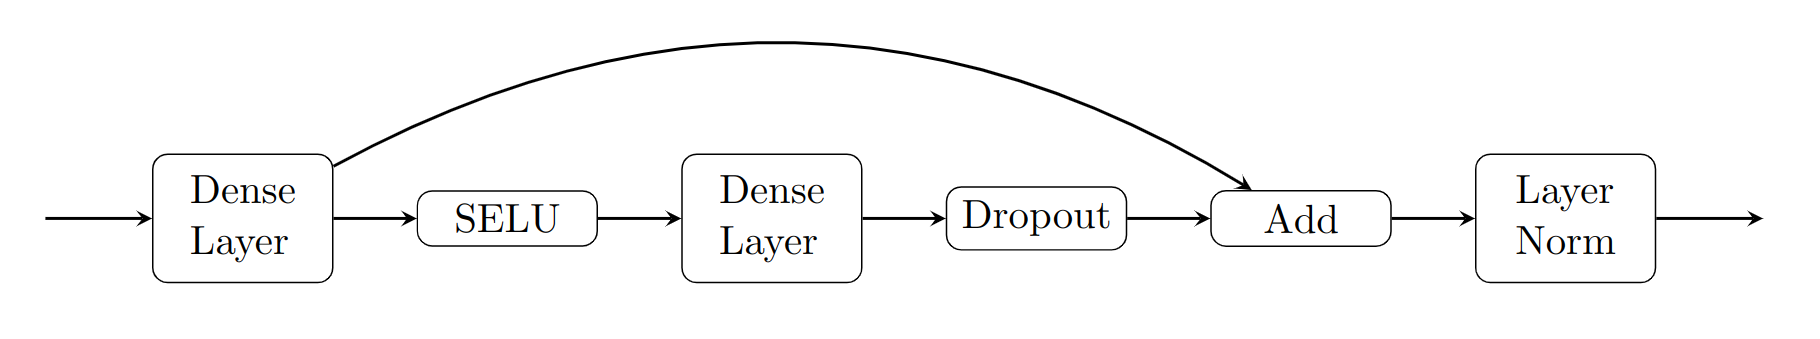
\includegraphics[width=1\linewidth]{img/Tikz_Model.png}
   \caption{\textit{Model Layout}}
\end{figure}  

\subsection{Loss Function Tweaks}
We made several attempts to refine the loss function while implementing various changes to the model in hopes of enhancing its performance.

\subsubsection{Contrastive Penalization}
Initially, we aimed to penalize the loss associated with similarities among distinct samples. This involved amplifying the loss tied to these similarities by a specified hyperparameter to further encourage the model to minimize similarities between different samples. Unfortunately, this approach proved unsuccessful, significantly compromising the model's performance.

\subsubsection{Weighted Loss}
Our subsequent attempt involved employing a weighted average strategy. In the original CLIP paper, the authors independently computed the loss for the image encoder and the text encoder, averaging these values. We attempted to improve this approach by weighting this average as follows: $\alpha \cdot L_{img} + (1 - \alpha) \cdot L_{txt}$. We experimented with both using $\alpha$ as a hyperparameter and as a trainable parameter (confined between 0 and 1). However, both attempts yielded no improvement. Interestingly, in the case of the trainable parameter, the resulting $\alpha$ value converged remarkably close to 0.5 after training. This indicated that employing a weighted average was futile, and a regular average remained the optimal choice.


\subsubsection{Geometric Mean}
Given that weighting the mean did not yield improvements, we experimented with various types of means for computing the final loss value, primarily focusing on the \textit{geometric mean}, represented in our case as: $\sqrt[2]{L_{img} \cdot L_{txt}}$. However, this attempt also proved unsuccessful, prompting us to retain the original formulation of the loss.

\subsection{Encoder Pre-training}
To enhance the stability of this intensive parameter training, we attempted to introduce a pre-training phase preceding the actual model training. The primary objective was to establish a more stable training process.

The approach involved pre-training the two encoders independently and without projections by incorporating a dense layer on top of them and training them in a multi-label classification scenario, making use of the provided concept dataset as labels. Subsequently, we would remove the dense classification layer and integrate the encoders into our CLIP model, followed by initiating the primary training phase.

Unfortunately, pre-training the text encoder did not yield any improvements; it only prolonged the entire training procedure. However, pre-training the image encoder resulted in a slight but consistent enhancement. Consequently, we opted to retain this initial pre-training for all subsequent iterations of the model.

\subsection{Data Augmentation}
To further improve performance we decided to insert data augmentation techniques inside our training and evaluation pipelines.
All the augmentation modules are given a seed for random number generation in order to improve the reproducibility of the process.

\subsubsection{Classic Data Augmentation}
Classic data augmentation (DAug) consists of adding minor perturbations of various natures on input training data in order to incentivize the model to generalize.
Due to the modular nature of our training pipeline, to implement the DAug process, it was sufficient to insert a map call in the dataset creation function, utilizing a dedicated parameter containing the DAug pipeline.

We experimented with various different DAug pipelines, but the following gave us best results:
\begin{figure}[H]
   \centering
   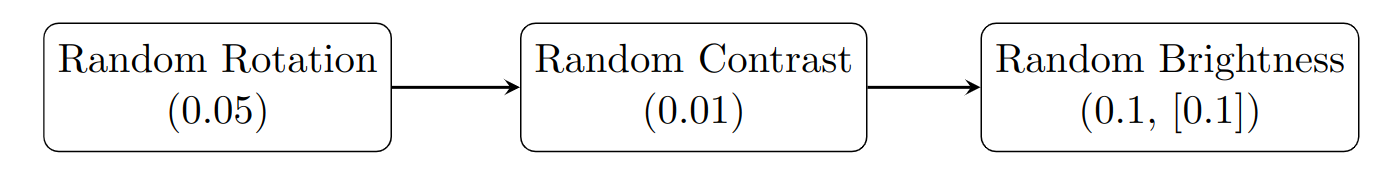
\includegraphics[width=1\linewidth]{img/Tikz_Daug_1.png}
   \caption{\textit{Image Pipeline}}
\end{figure}
\begin{figure}[H]
   \centering
   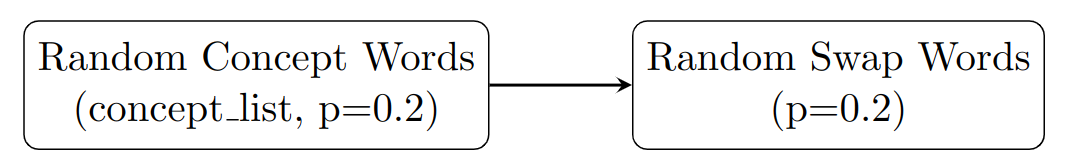
\includegraphics[width=0.8\linewidth]{img/Tikz_Daug_2.png}
   \caption{\textit{Text Pipeline}}
\end{figure}

All the image augmentation modules are provided by the \href{https://www.tensorflow.org/api_docs/python/tf/keras/layers/}{Keras Layers} library and their parameters generally correspond to symmetric transformation ranges (except for the Random Brightness layer, where the first parameter is the factor range and the second parameter is the value range).

The text augmentation modules were implemented by us, drawing inspiration from the \href{https://www.kaggle.com/code/shonenkov/nlp-albumentations}{NLP Albumentations notebook} by Alex Shonenkov.
The \texttt{RandomSwapWords} module takes a probability $p$ as parameter, and with that probability creates a boolean mask for the caption associated with a certain input sample. The words highlighted by the mask are then randomly shuffled.
The \texttt{RandomConceptWords} module takes a list of concept classes and a probability $p$ as parameters, selects a random number of concepts based on $p$ and the concepts of the input sample, randomly selects a position inside the caption for each selected concept, and inserts the concept reference texts inside the caption at the chosen positions.

Even though the direct increase in performance caused by DAug was marginal, it opened up other paths for improvement that were previously unfeasible due to the model overfitting, such as using a larger BERT architectures and employing a bigger embedding size.

\subsubsection{Test Time Augmentation}
Test Time Augmentation (TTA) is slightly different from DAug, as it is performed inside the model, at inference time.
In order to reduce variance of predictions, the model is given \texttt{tta\_n} different augmented versions of the same input sample (plus the original inputs), the model is asked to perform a prediction for all of them, and then average the results to obtain a final prediction.

For TTA we utilized the same augmentation pipeline as in the previous step, with slightly modified parameters to make it more aggressive and without the \texttt{RandomConceptWords} module.
We then implemented a wrapper for the encoders of the model, that takes as input the actual encoder of the model, an augmentation pipeline, and other TTA parameters (such as \texttt{tta\_n}). The wrapper produces a modified encoder that performs TTA with the desired parameters whenever is called.

Unfortunately there were no direct improvements by using TTA, at best it resulting in a performance equivalent to the base model.
With TTA being a self-ensembling method, our guess is that the model is too stable on its predictions to gain any meaningful benefit from this technique.

\subsection{Grayscale Preprocess}
We noticed that most of the images contained in the dataset are grayscale images. However, they are stored as RGB images, with a shape of $ 128 \times 128 \times 3 $. Being grayscale, the third dimension is completely redundant, and we know that additional dimensions can severely impact the model's performance. To address this, we implemented a solution by introducing a \href{https://www.tensorflow.org/api_docs/python/tf/keras/layers/Lambda}{Lambda layer} at the beginning of the image encoder. This layer calculates the average across the RGB channels (the third dimension) for inputs with three dimensions, effectively creating a simple color-to-grayscale conversion algorithm that outputs a 2-dimensional image. For inputs already in grayscale with two dimensions, the layer remains inactive.

This modification ensures seamless compatibility of the encoder with our existing infrastructure, requiring no alterations. Consequently, our model can effectively process both grayscale and RGB inputs. This way, our image encoder now operates on dimensions of $128 \times 128$.

The integration of this solution had a significant positive impact on the model's performance, resulting in substantial improvement.

\subsection{Evaluation}
In the first steps of this project we were using the \textit{loss} returned by the model as its quality metric, which is not really optimal for various reasons, therefore we decided to write a separate notebook solely dedicated to model evaluation for the two main retrieval tasks.
An additional similar notebook was created with the purpose of comparing multiple models' performance on the established evaluation metrics.

The inference procedure is specular for image and text retrieval: we first generate the embeddings of the feature that we want to retrieve by calling the \texttt{predict} method of the relevant encoder on the dataset that we want to utilize.
Then, for every query of the dataset we generate the embedding through the other encoder, and we compute the \textit{cosine similarity} to then retrieve the \textit{top-k} results for each query.

Finally, we compute the mean \textbf{accuracy}, \textbf{precision}, \textbf{recall} and \textbf{F1 score} for the query dataset through \textit{micro-averaging}, and we visualize them utilizing \textit{graphs} and \textit{reports} with the possibility of comparing evaluations between models or against a random classifier baseline.
However, we noticed there are multiple \textbf{relevance metrics} that are interesting to take into consideration (for simplicity, only image retrieval is illustrated):
\begin{itemize}
   \item \textbf{Caption Equality}: a result is relevant only if its caption is equal to the original query; it can be quite restrictive since most of the captions are unique.
   \item \textbf{Concept Overlap}: a result is relevant only if it shares \textit{n} concepts with the original element; it provides a good estimate for real use-cases but can be misleading if the threshold is too low, in addition it cannot be used if the concept data is not present.
\end{itemize}

Some other evaluation approaches were tried for the image retrieval scenario, such as the \textit{Concept-Fusion Captions} approach, which consists of evaluating the model on samples where each caption was generated by concatenating the concepts of the corresponding sample.
This method of evaluation steadily gave worse results than other approaches.


%------------------------------------------------------------------------
\section{Results}

\subsection{Image and Text Retrieval Samples}
Some sample outputs from the image and text retrieval tasks using $k=3$.

For visualization reasons, both image and text data is shown in the results of both retrieval tasks; only the target feature is actually retrieved by the model in each task, while the other is obtained through a lookup of the dataset.

\begin{figure}[H]
    \centering
    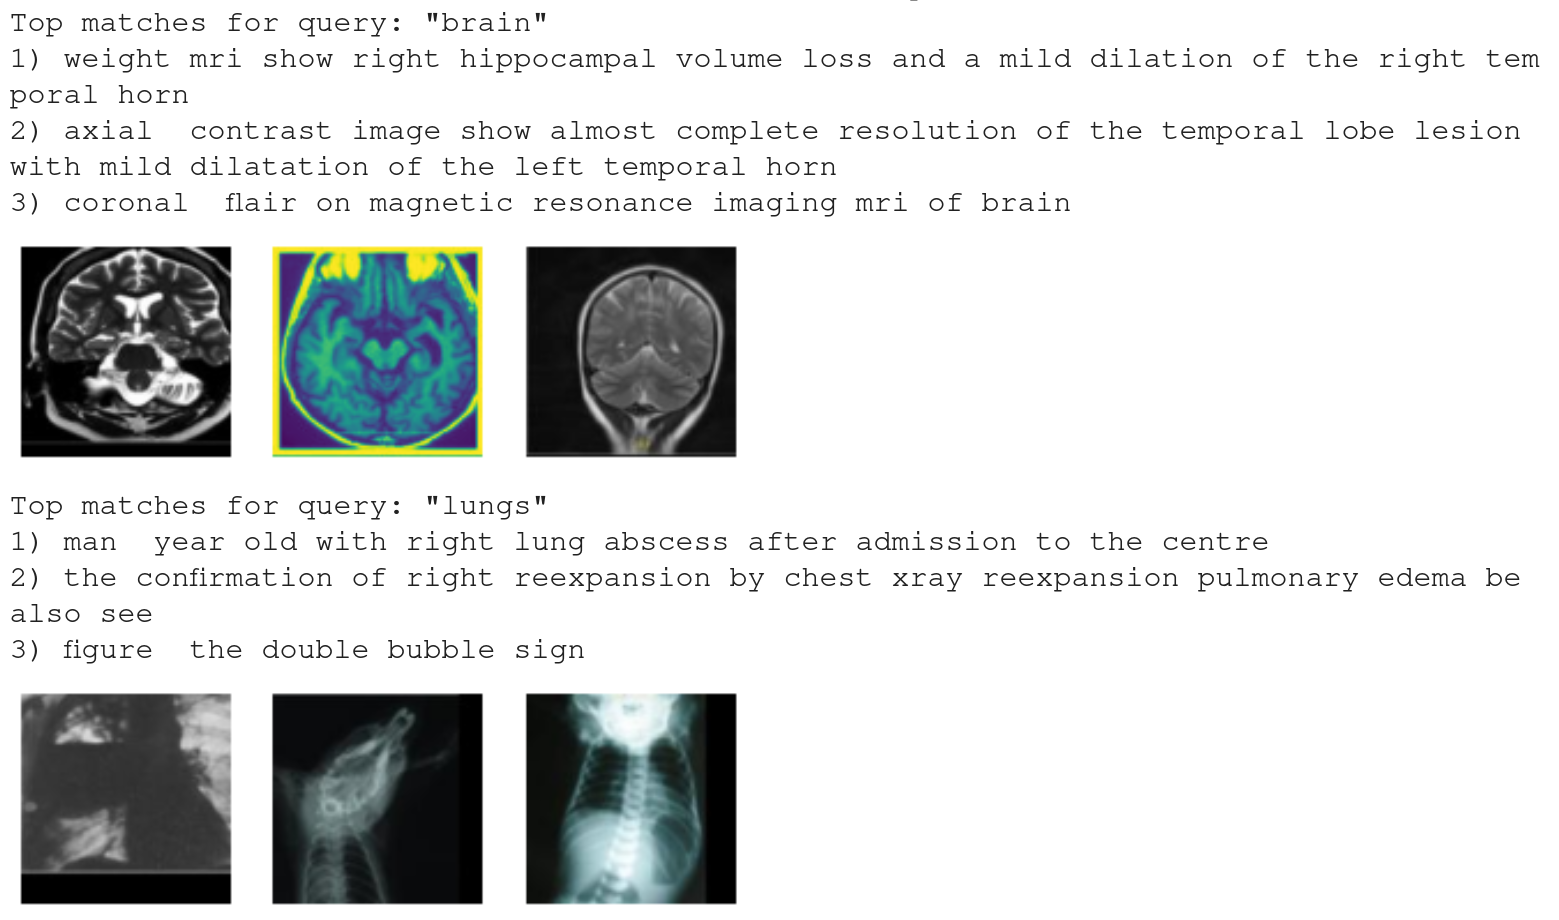
\includegraphics[width=1\linewidth]{img/T2I_test1.png}
    \caption{\textit{Image Retrieval}}
\end{figure}

\begin{figure}[H]
   \centering
   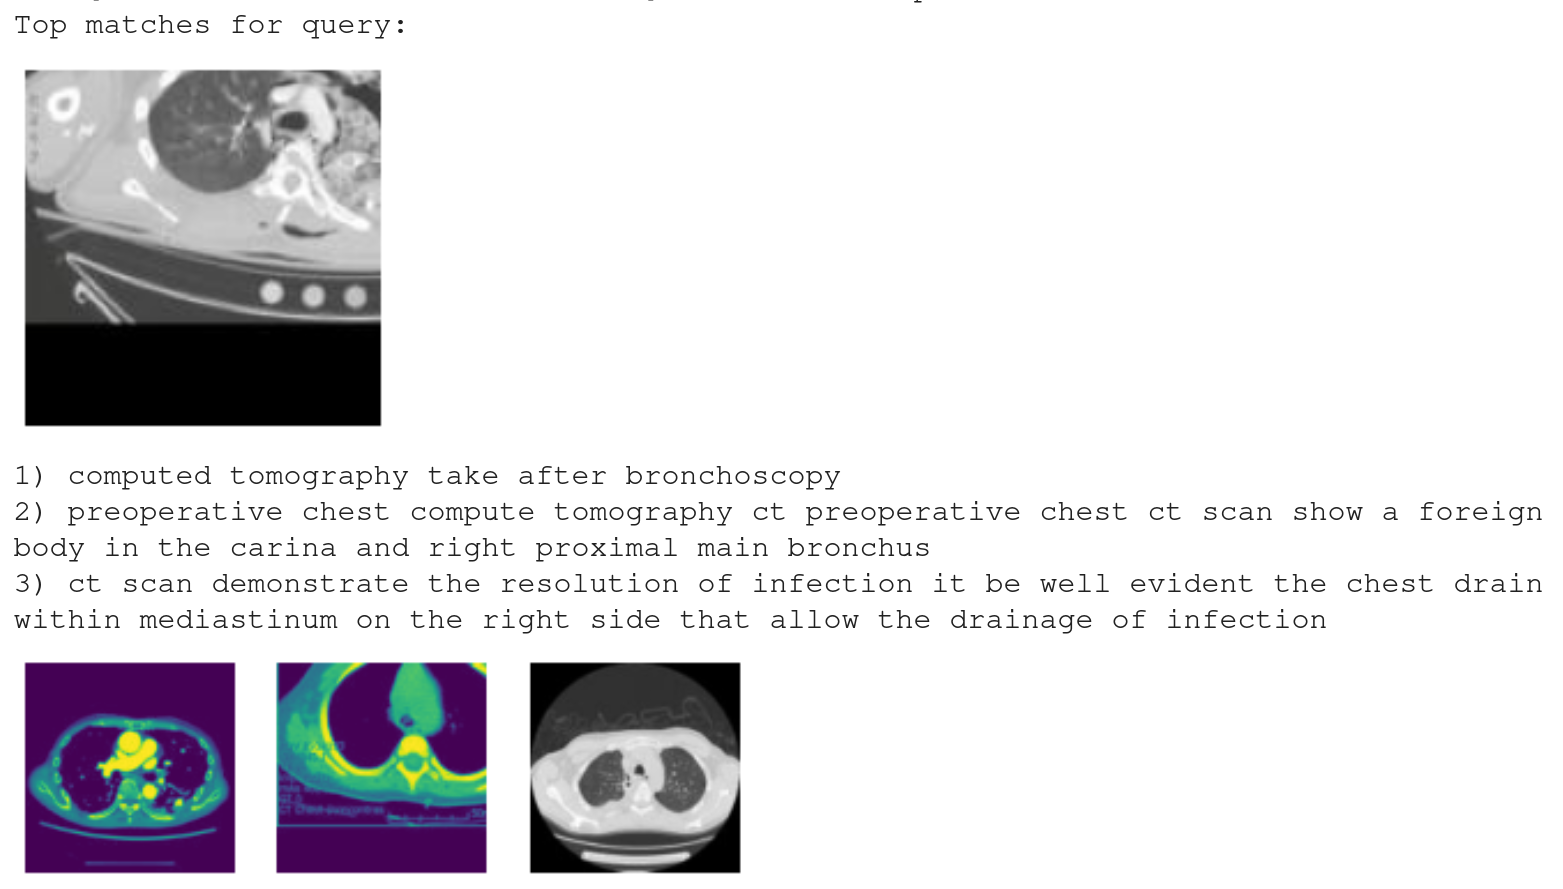
\includegraphics[width=1\linewidth]{img/I2T_test1.png}
   \caption{\textit{Text Retrieval 1}}
\end{figure}
\begin{figure}[H]
   \centering
   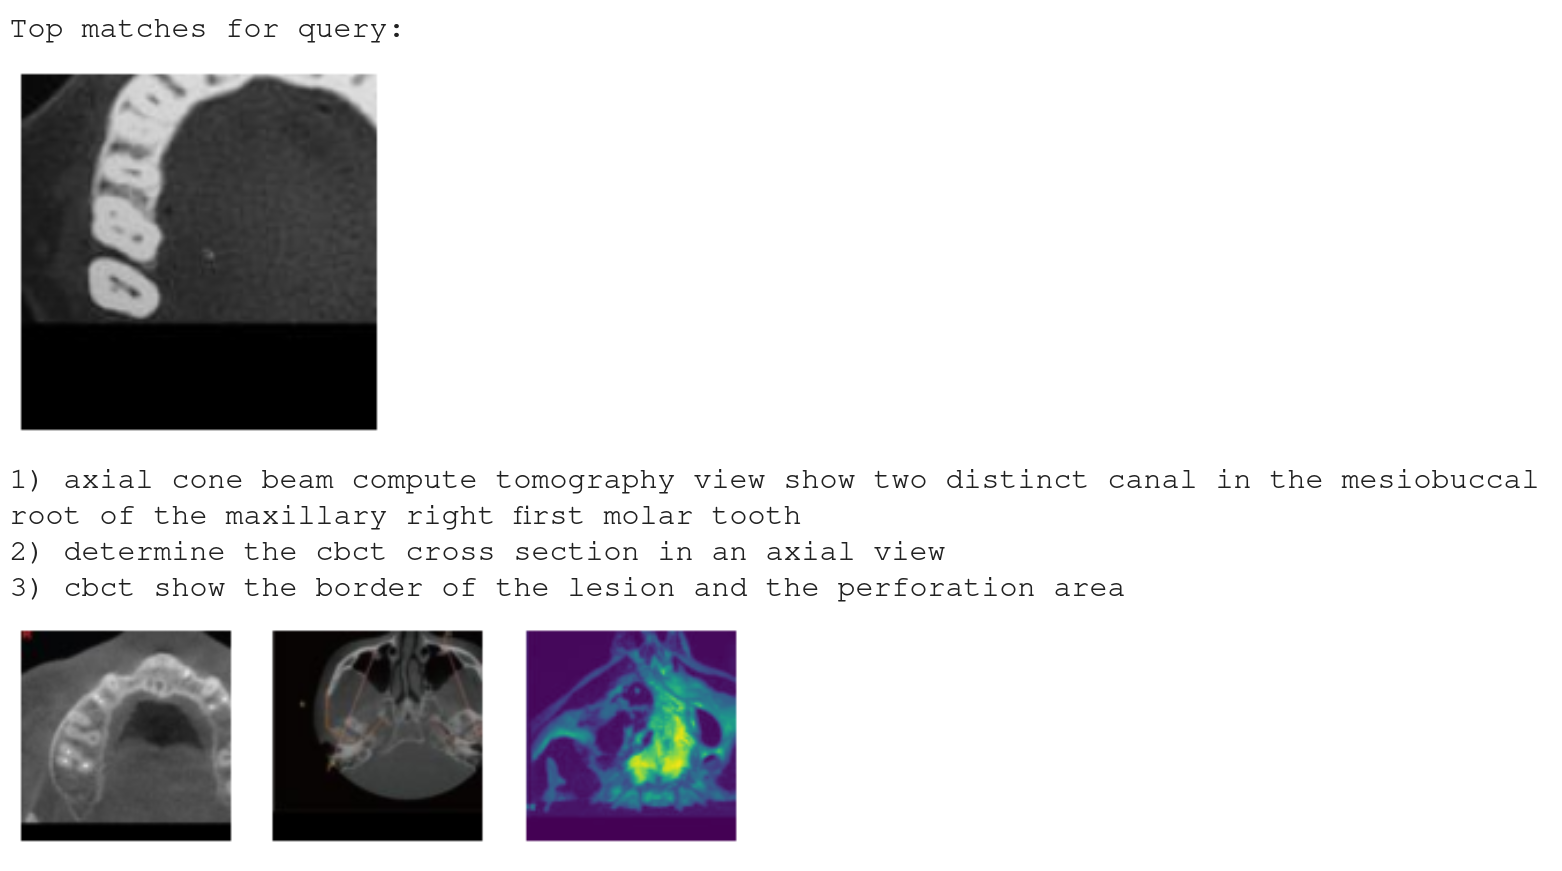
\includegraphics[width=1\linewidth]{img/I2T_test2.png}
   \caption{\textit{Text Retrieval 2}}
\end{figure}

\subsection{Model Architecture Improvement}

The final iteration of the model emerged after implementing various tweaks and adjustments to its architecture and training methods mentioned in the previous section. However, not all of them resulted in an improved model. Some changes led to worse outcomes, while others showed no discernible impact. Each adjustment underwent meticulous evaluation using the methodologies mentioned before (\textit{caption equality} and \textit{concept overlap}). Given the numerous changes to the model and the many more evaluation results for each, we have summarized the overall enhancement of the model through a corresponding chart.

This chart displays the \textbf{concept overlap accuracy} at $k=10$ and with a concept threshold of $n=2$ for each model modification, as it serves as a concise and clear metric to show the progression. Blue bars on the chart signify changes that yielded improvements in the architecture and were consequently integrated, while gray bars indicate changes that failed to enhance the model and were thus discarded.

\begin{figure}[H]
    \centering
    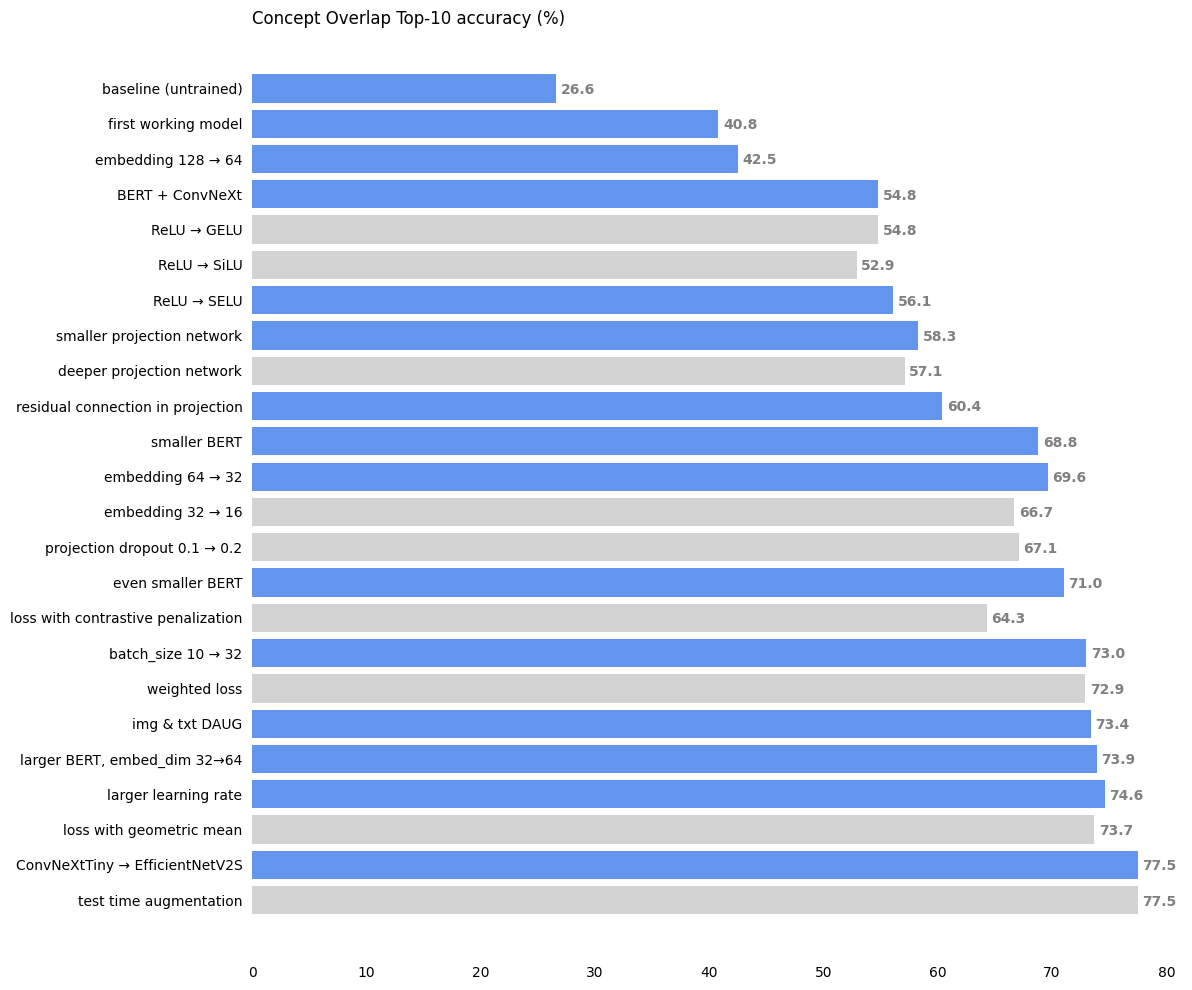
\includegraphics[width=1\linewidth]{img/Improvement_Plot.png}
    \caption{\textit{Model improvement overview}}
\end{figure}

\subsection{Embedding Space}

To effectively demonstrate the model's capabilities and the coherence of its \textit{embedding space}, our aim now is to visualize its inner workings, specifically how the \textit{visual encoder} and the \textit{text encoder} interact. The primary goal of the model is centered on training both encoders to encode images and their corresponding descriptions within a unified embedding space. This process generates two latent vectors (one for images and one for captions) that ideally exhibit high similarity to each other while remaining distinct from other sample pairs within the set.

To illustrate this concept, we selected a random batch of 32 samples from the test dataset.
We then employed their respective encoders to encode both the images and their associated captions.
Subsequently, we normalized these embeddings and computed similarities by performing matrix multiplication between them. This process allows us to quantify the relationships and similarities between the encoded representations of images and captions within this shared embedding space on data that the model has never seen.

\begin{figure}[H]
   \centering
   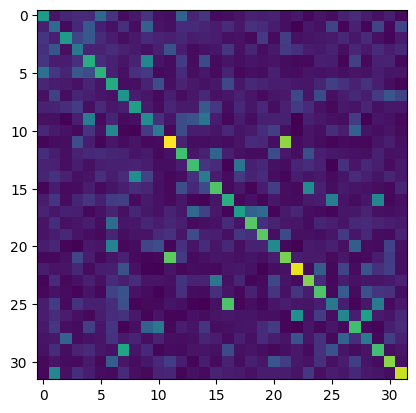
\includegraphics[width=0.6\linewidth]{img/Diagonal.png}
   \caption{\textit{Diagonal rend in embeddings}}
\end{figure}

As expected, our observations reveal a clear \textit{diagonal trend} within the visualization.
This trend distinctly illustrates that images and captions originating from the same sample show a notably high degree of similarity, denoted by a brighter color in the visualization.
Conversely, when comparing images and captions from different samples, the similarity appears significantly lower, depicted by a darker color.


%------------------------------------------------------------------------
\section{Zero-Shot Image Classification}

Once our model had successfully achieved a high level of performance, we decided to put it to the test in a \textit{zero-shot classification} scenario, as demonstrated and utilized in the CLIP paper.

The fundamental idea behind this approach involves having a set of textual classes serving as our classification labels. When presented with an image for classification, we encode both the image and the classes. Following this, we calculate the similarity between the embedding of the image and the embeddings of the classes. By applying a \textit{softmax function} in order to sharpen the distribution, we determine the highest similarity score, which becomes our prediction.

\subsection{Custom Dataset}
In order to comprehensively assess our model's classification capabilities, we opted to construct a tailored dataset specifically designed for this purpose. Our rationale came from the observation that nearly every entry in the dataset caption explicitly delineated the type of analysis depicted in the corresponding image, such as \textit{`x-ray scan of\ldots'} or \textit{ `ultrasound image of\ldots}'. Hence, we decided to create a dataset where each sample comprised an image paired with a label representing the specific type of analysis conducted in that image.

To create this dataset, we utilized our test dataset, to avoid any potential biases. We built a piece of code to extract words from a predefined set of labels found within the image captions. These labels were subsequently employed as classes, allowing us to compile a custom dataset. The chosen classes are: \textbf{angiography, echocardiography, ultrasound, tomography, x-ray}.

Upon extracting the images from the test set, we ended up with a dataset comprising 4111 samples, with each sample associated with one of the specified five labels, with the following class distribution of samples: angiography: \textit{299}, echocardiography: \textit{211}, ultrasound: \textit{520}, tomography: \textit{1873}, xray: \textit{1208}.

\subsection{Results}

\begin{figure}[H]
   \centering
   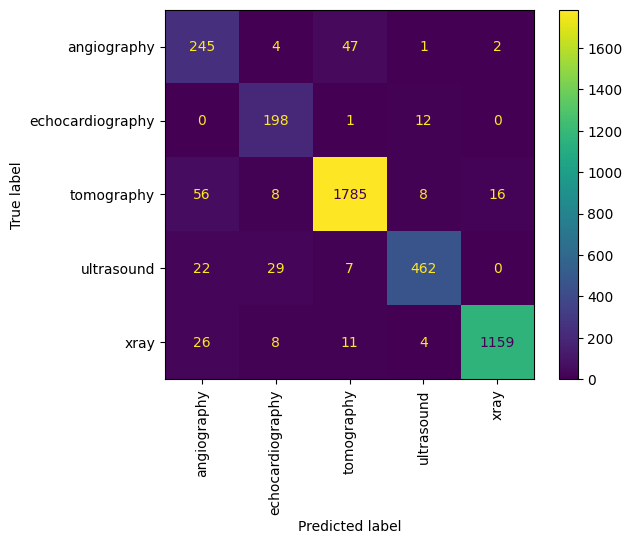
\includegraphics[width=1\linewidth]{img/Classification_Result.png}
   \caption{\textit{Classification Confusion Matrix}}
\end{figure}

We then wrapped the classification procedure in a function and performed evaluation just as we would normally do with a trained classifier.

As it's possible to observe from the confusion matrix visualization, the model's predictions seem well-balanced as a faint diagonal is present.
However, there might be some slight bias towards the \textit{angiography class} as it is the one with the most false positive predictions associated overall.
This is possibly due to the conceptual overlap between the angiography technique and other types of exams such as x-ray and tomography.

These results led to an overall \textbf{accuracy} of \textbf{94\%}, exceeding our brightest expectations.


%------------------------------------------------------------------------
\section{Conclusions}
TODO Conclusions.\cite{steinhardt, lipton}

%-------------------------------------------------------------------------

{\small
\bibliographystyle{bib/ieee}
\bibliography{bib/egbib}
}

\end{document}
